% Preamble
\documentclass[12pt, a4paper]{article}
\title{\emph{Best Books for Human\\Emotions} \& \emph{Disorders}}
\author{Written by Volunteers}
\date{July 12, 2021}

% Packages
\usepackage{sectsty}
\usepackage{xcolor}
\usepackage{caption}
\usepackage[utf8]{inputenc}
\usepackage{hyperref}
\usepackage{graphicx}
\graphicspath{{images/}}

% Settings
\sectionfont{\Huge\itshape}%
\subsectionfont{\Large\itshape}%
\subsubsectionfont{\itshape}%

% Macros
\newcommand{\nl}{\vspace{\baselineskip}}

% Body
\begin{document}
\maketitle
\begin{enumerate}

\item Social Skills
\item Generalized Anxiety Disorder
\item Social Anxiety Disorder \& Shyness
\item Overthinking
\item Jealousy
\item Self-awareness
\item Self-consciousness
\item Happiness
\item Paranoia
\item Revenge
\item Self-confidence / Self-esteem
\item False Self-confidence / Self-esteem
\item Addiction
\item OCD
\item Perfectionism
\item Child Abuse
\item Painful Past
\item Panic Attack
\item Self-harm / Self-injury
\item Suicide
\item Trauma
\item Post Traumatic Stress Disorder
\item Shizoaffective
\item Shizophernia
\item Hallucinations
\item Delusional Disorder
\item Major Depressive Disorder
\item Dysthymia
\item Bipolar Disorder

\end{enumerate}

\begin{center}
	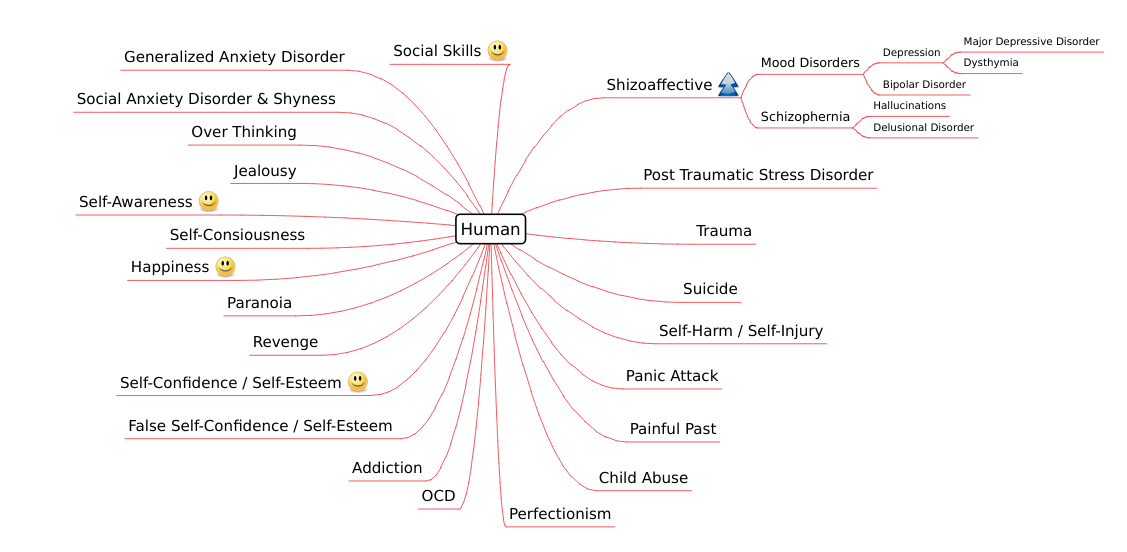
\includegraphics[scale=0.43]{human.png}
\end{center}

\newpage

\begin{large}
\paragraph{}
If you want to contribute, read these considerations:

\begin{enumerate}

\item The author should have a PhD degree in related topic
\item The author should be an expert in that field
\item The author's methods must be applicable

\end{enumerate}

\end{large}

\newpage

% Social Skills
\section*{Social Skills}
\subsubsection*{The Social Skills Guide Book}
\subsubsection*{How to Win Friends and Influence People}
\subsubsection*{Conversationally Speaking}
\subsubsection*{How to Speak, How to Listen}\nl
\subsection*{* Additional *}
\subsubsection*{Improve your Social Skills}\nl


% Generalized Anxiety Disorder
\section*{Generalized Anxiety Disorder}
\subsubsection*{Generalized Anxiety Disorder Work Book: A Comprehensive CBT Guide}
\subsubsection*{Rewire your Anxious Brain}\nl
\subsection*{* Additional *}
\subsubsection*{Cognitive Behavioral Anxiety Disorder Treatment for Generalized}
\subsubsection*{The Anxiety and Worry Workbook: The Cognitive Behavioural Solution}
\subsubsection*{Generalized Anxiety Disorder: Advances in Research and Practice}\nl

% Social Anxiety Disorder & Shyness
\section*{Social Anxiety Disorder \& Shyness}
\subsubsection*{The Shyness \& Social Anxiety Workbook}
\subsubsection*{Overcoming Social Anxiety \& Shyness}\nl

\newpage

% Overthinking
\section*{Overthinking}
\subsubsection*{The Worry Trick}
\subsubsection*{Soundtracks: The Surprising Solution to Overthinking}\nl

% Self-confidence / Self-esteem
\section*{Self-confidence / Self-esteem}
\subsubsection*{The Confidence Gap}
\subsubsection*{The Self-confidence Workbook}\nl

\subsection*{* Additional *}
\subsubsection*{Self-esteem: A Proven Program of Cognitive Technique}
\subsubsection*{How to be yourself}\nl







\end{document}
